\documentclass[12pt]{article}
\usepackage{graphicx} % Required for inserting images

\linespread{1.1} % for more than single spacing

% take more advantage of the size of paper
\addtolength{\topmargin}{-2cm}
\addtolength{\textheight}{4cm}
\addtolength{\evensidemargin}{-2cm}
\addtolength{\oddsidemargin}{-2cm}
\addtolength{\textwidth}{4cm}

% some standard packages
\usepackage{mathalpha}
\usepackage{times}
\usepackage{graphics, graphicx}
\usepackage{subfigure, epsfig}
\usepackage{rotate}
\usepackage{tikz, amsmath, amssymb}
\usepackage{enumitem}
\usepackage{hyperref}
\usepackage{float} % for forcing position of figures with H
\usepackage{listings} % for code and output embedding
\lstdefinestyle{mystyle}{
    basicstyle=\ttfamily\footnotesize
}
\lstset{style=mystyle}

% convenient abbreviations
\newcommand{\Cee}{\mathbf{C}}
\newcommand{\Iee}{\mathbf{I}}
\newcommand{\Lee}{\mathbf{L}}
\newcommand{\Ccal}{\mathcal{C}}
\newcommand{\Ical}{\mathcal{I}}
\newcommand{\Lcal}{\mathcal{L}}
\newcommand{\mc}{\multicolumn}
\newcommand{\hs}{\hspace}
\newcommand{\EQ}{\begin{equation}}
\newcommand{\EN}{\end{equation}}
\newcommand{\EQA}{\begin{eqnarray}}
\newcommand{\ENA}{\end{eqnarray}}
\newcommand{\EQAS}{\begin{eqnarray*}}
\newcommand{\ENAS}{\end{eqnarray*}}
\title{CSC311 Report}
\author{Linda Cai, Shizhao Zheng, Yuhan Fu, Yufei Chen}
\date{April 2024}

\begin{document}

\maketitle
\section*{Part A}
\subsection*{1. KNN}
\subsubsection*{(a)}
\subsubsection*{(b)}
\subsubsection*{(c)}
\subsubsection*{(d)}
\subsubsection*{(e)}

\newpage
\subsection*{2. Item Response}
\subsubsection*{(a)}
\begin{align*}
p(C|\theta,\beta) &= \prod_{i,j} \left( p(C_{ij}=1|\theta_i,\beta_j) \right)^{C_{ij}} \left(p(C_{ij}=0|\theta_i,\beta_j) \right)^{1 - C_{ij}}
\end{align*}
\begin{align*}
\log p(C|\theta,\beta) &= \sum_{i,j} C_{ij} \log \left( p(C_{ij}=1|\theta_i,\beta_j) \right) + (1 - C_{ij}) \log \left( 1 - p(C_{ij}=1|\theta_i,\beta_j) \right) \\
&= \sum_{i,j} C_{ij} \log \left( \frac{\exp(\theta_i - \beta_j)}{1 + \exp(\theta_i - \beta_j)} \right) + (1 - C_{ij}) \log \left( 1 - \frac{\exp(\theta_i - \beta_j)}{1 + \exp(\theta_i - \beta_j)} \right) \\
&= \sum_{i,j} C_{ij} (\theta_i - \beta_j) - \sum_{i,j} \log(1 + \exp(\theta_i - \beta_j)) \\
&\quad + \sum_{i,j} \log(1 + \exp(\theta_i - \beta_j)) - \sum_{i,j} C_{ij} \log(1 + \exp(\theta_i - \beta_j)) \\
&= \sum_{i,j} C_{ij} (\theta_i - \beta_j) - \sum_{i,j} C_{ij} \log(1 + \exp(\theta_i - \beta_j))\\
&=\sigma(\theta, \beta)
\end{align*}
$$\frac{\partial}{\partial \theta_i} \log p(C|\theta,\beta) = \sum_{j} C_{ij} - \sum_{j} \frac{\exp(\theta_i - \beta_j)}{1 + \exp(\theta_i - \beta_j)}$$
$$\frac{\partial}{\partial \beta_j} \log p(C|\theta,\beta) = - \sum_{i} C_{ij} + \sum_{i} \frac{\exp(\theta_i - \beta_j)}{1 + \exp(\theta_i - \beta_j)}
$$
\subsubsection*{(c)}


\subsubsection*{(d)}


\newpage
\subsection*{3. Matrix Factorization}
\subsubsection*{(a)}
I ran SVD with k = 1, 2, 5, 10, 20 and calculated the validation accuracy for each k. The best k was 5 with an accuracy of 0.659046006209427.\\
Validation Accuracy: 0.6428168219023427 with k = 1\\
Validation Accuracy: 0.6579170194750211 with k = 2\\
Validation Accuracy: 0.659046006209427 with k = 5\\
Validation Accuracy: 0.6586226361840248 with k = 10\\
Validation Accuracy: 0.6539655659046006 with k = 20\\
So k = 5 is chosen as the best k,with validation accuracy 0.659046006209427.\\
Best k: 5 with test accuracy: 0.6635619531470506\\

\subsubsection*{(b)}
One limitation of SVD for this task is that it treats missing entries by using mean imputation. However,
mean imputation can introduce noise, especially in sparse regions of the data, as it assumes that missing values are similar
to the mean of the respective item. This might not hold true in reality, especially for different users or items. Therefore,
a limitation of SVD in this case is that it may lead to incorrect estimations of missing values, thereby affecting the quality
of matrix reconstruction.


\subsubsection*{(c \& d)}
After implementing the ALS with SGD, I ran the algorithm with k = 1, 2, 5, 10, 20,lr = 0.01, 0.1, 0.5, 1, iterations from 1 to 1000 with step size 20.\\
Finally, I found the best k = 1,lr = 0.5, iterations =361 is the best set of hyperparameters.\\
\subsubsection*{(e)}
%添加图片
\begin{figure}[h]
\centering
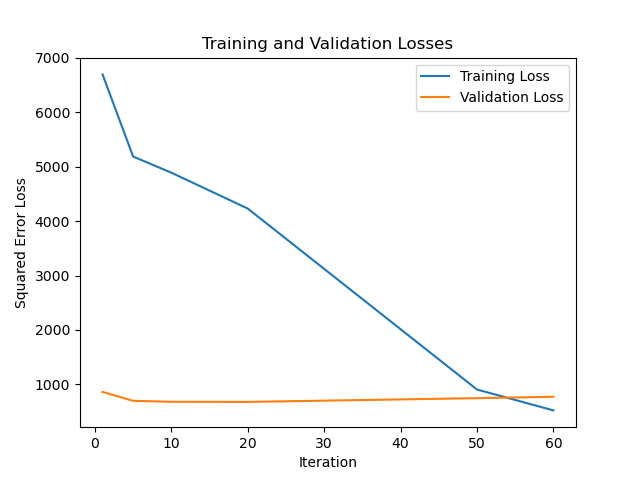
\includegraphics[width=0.5\textwidth]{losses vs iteration.png}
\caption{Losses vs Iteration}
\end{figure}
final model is trained with k = 1,lr = 0.5, iterations =361 with validation accuracy 0.44919559695173583, test accuracy 0.46316680779000846.\\

\newpage
\section*{Part B}
\subsection*{1. Formal Description of Modified Algorithm}

\subsection*{2. Figures and Diagrams of Modified Algorithm}

\subsection*{3. Comparing Modified Model with Baseline Model}

\subsection*{4. Explanation of Model's Performance}

\subsection*{5. One Limitation of the Model}

\end{document}
